\section{Mekanisme Panggilan: Konvensi Register}

Prosedur pemanggilan fungsi melibatkan pembagian tanggung jawab antara fungsi yang memanggil (\textit{caller}) dan fungsi yang dipanggil (\textit{callee}) dalam mengelola register CPU.

\subsection{Caller-Saved vs Callee-Saved}
Kompilator menggunakan konvensi berikut untuk menjaga integritas data:
\begin{enumerate}
    \item \textbf{Caller-Saved Registers} (Volatile): Register yang nilainya boleh dirusak oleh fungsi yang dipanggil. Jika \textit{caller} membutuhkan nilai di register ini setelah panggilan fungsi, \textit{caller} harus menyimpannya ke stack sebelum perintah \code{call}. Contoh pada x86-64: \texttt{rax}, \texttt{rcx}, \texttt{rdx}.
    \item \textbf{Callee-Saved Registers} (Non-volatile): Register yang nilainya harus tetap sama bagi \textit{caller} sebelum dan sesudah panggilan. Jika \textit{callee} ingin menggunakan register ini, ia harus menyimpan isinya di awal fungsi (\textit{prologue}) dan memulihkannya di akhir fungsi (\textit{epilogue}). Contoh pada x86-64: \texttt{rbx}, \texttt{rbp}, \texttt{r12-r15}.
\end{enumerate}

\subsection{Penyaluran Parameter}
Pada arsitektur modern (seperti System V AMD64 ABI), enam parameter pertama biasanya dikirim melalui register (\texttt{rdi, rsi, rdx, rcx, r8, r9}) alih-alih stack untuk meningkatkan performa. Parameter ke-7 dan seterusnya baru dikirim melalui stack.

\begin{figure}[!htbp]
    \centering
    \adjustbox{max width=0.8\textwidth,center}{%
    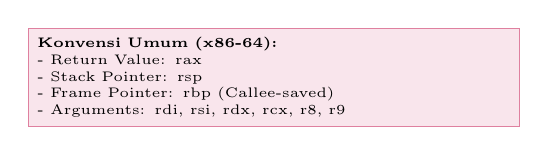
\begin{tikzpicture}[
        rect/.style={rectangle, draw=purple!50, fill=purple!10, text width=6cm, font=\tiny}
    ]
    \node[rect] (reg) {
        \textbf{Konvensi Umum (x86-64):}\\
        - Return Value: \code{rax}\\
        - Stack Pointer: \code{rsp}\\
        - Frame Pointer: \code{rbp} (Callee-saved)\\
        - Arguments: rdi, rsi, rdx, rcx, r8, r9
    };
    \end{tikzpicture}%
    }
    \caption{Peta Penggunaan Register dalam Prosedur Panggilan}
\end{figure}
